%%
%% Copyright 2007, 2008, 2009 Elsevier Ltd
%%
%% This file is part of the 'Elsarticle Bundle'.
%% ---------------------------------------------
%%
%% It may be distributed under the conditions of the LaTeX Project Public
%% License, either version 1.2 of this license or (at your option) any
%% later version.  The latest version of this license is in
%%    http://www.latex-project.org/lppl.txt
%% and version 1.2 or later is part of all distributions of LaTeX
%% version 1999/12/01 or later.
%%
%% The list of all files belonging to the 'Elsarticle Bundle' is
%% given in the file `manifest.txt'.
%%

%% Template article for Elsevier's document class `elsarticle'
%% with numbered style bibliographic references
%% SP 2008/03/01
%%
%%
%%
%% $Id: elsarticle-template-num.tex 4 2009-10-24 08:22:58Z rishi $
%%
%%
%%\documentclass[preprint,12pt,3p]{elsarticle}
\documentclass[12pt,3p]{elsarticle}
%% Use the option review to obtain double line spacing
%% \documentclass[preprint,review,12pt]{elsarticle}

%% Use the options 1p,twocolumn; 3p; 3p,twocolumn; 5p; or 5p,twocolumn
%% for a journal layout:
%% \documentclass[final,1p,times]{elsarticle}
%% \documentclass[final,1p,times,twocolumn]{elsarticle}
%% \documentclass[final,3p,times]{elsarticle}
%% \documentclass[final,3p,times,twocolumn]{elsarticle}
%% \documentclass[final,5p,times]{elsarticle}
%% \documentclass[final,5p,times,twocolumn]{elsarticle}

%% if you use PostScript figures in your article
%% use the graphics package for simple commands
%% \usepackage{graphics}
%% or use the graphicx package for more complicated commands
%% \usepackage{graphicx}
%% or use the epsfig package if you prefer to use the old commands
%% \usepackage{epsfig}

%% The amssymb package provides various useful mathematical symbols
\usepackage{amssymb}
\usepackage[spanish]{babel}
\usepackage[utf8]{inputenc}
\usepackage{graphicx}
\usepackage{amsmath}
\usepackage{subfigure} 
\usepackage{float}
% For algorithms
\usepackage{algorithm}
\usepackage{algorithmic}


%% The amsthm package provides extended theorem environments
%% \usepackage{amsthm}

%% The lineno packages adds line numbers. Start line numbering with
%% \begin{linenumbers}, end it with \end{linenumbers}. Or switch it on
%% for the whole article with \linenumbers after \end{frontmatter}.
%% \usepackage{lineno}

%% natbib.sty is loaded by default. However, natbib options can be
%% provided with \biboptions{...} command. Following options are
%% valid:

%%   round  -  round parentheses are used (default)
%%   square -  square brackets are used   [option]
%%   curly  -  curly braces are used      {option}
%%   angle  -  angle brackets are used    <option>
%%   semicolon  -  multiple citations separated by semi-colon
%%   colon  - same as semicolon, an earlier confusion
%%   comma  -  separated by comma
%%   numbers-  selects numerical citations
%%   super  -  numerical citations as superscripts
%%   sort   -  sorts multiple citations according to order in ref. list
%%   sort&compress   -  like sort, but also compresses numerical citations
%%   compress - compresses without sorting
%%
%% \biboptions{comma,round}

% \biboptions{}


\journal{--}

\begin{document}

\begin{frontmatter}

\title{Análisis del Generador Renyi Map.}



\author{Marcos Daniel Calderón Calderón}



\ead{marcos.calderon@cimat.mx}




\begin{abstract}
En este reporte, se hacen algunas pruebas del tamaño de ciclo del mapa caótico Renyi. 
\end{abstract}

%\begin{keyword}
%% keywords here, in the form: keyword \sep keyword
%Mapa  \sep \LaTeX \sep Generador no lineal

%\end{keyword}

\end{frontmatter}

\section{Características a tomar en cuenta para la realización de las pruebas.}

\begin{enumerate}
\item Siempre ocurrió que $ j \geq n$ para que el mapa se comporte como un generador congruencial lineal (LCG). 

\item Otra cosa que se debe de tener en cuenta es lo siguiente, al igual que en las pruebas del paper, es necesario que $i=j$. 

\item Ahora, lo que hacemos es definir el valor de q como $impar$.


\end{enumerate}

Con las características mencionadas arriba, lo que se busca es obtener un período máximo de $2^{n}-1$. De acuerdo a diversos estudios realizados, para obtenener un tamaño máximo de ciclo, es necesario que la función sea invertible (biyectiva y suprayectiva). Esto sólo se logra si $i=j$. 

La proposición 1 del artículo  \cite{Addabbo} demuestra que el mapa caótico Renyi es invertible cuando $i=j$,  y que si cumple esta condición, es posible encontrar siclos de tamaño máximo.

Además, al utilizar $i=j =n$, obtenemos una simplificación del mapa caótico:

\begin{equation}
f(k)= qk \mod{2^{n}}
\end{equation}
 





\begin{enumerate}
\item \textbf{unsigned long} Es un tipo de dato utilizado en C, es una variable para almacenar números en 32 bits (4 bytes). Por el contrario que las variables long estándar, las unsigned long no almacenan números negativos, haciendo que su rango sea de 0 a 4,294,967,295 ($2^{32} - 1$).


\item \textbf{Máscaras.} Son secuencias de bits que tienen la finalidad de ocultar o mostrar bits específicos de otra secuencia de bits. Esto se logra al aplicar un operador lógico a la máscara con la secuencia original.

\item \textbf{Hexadecimales en C.} La representación de Hexadecimales en C se realiza al anteponer los caracteres ''0x'' al número que estará en Hexadecimal.

\item \textbf{Operacion módulo en bits.} A la hora de utilizar esta operación en generación de números pseudoaleatorios, se utiliza la operación lógica de $ \& $ con una máscara de bits. 

\end{enumerate}

\section{Resultados.}




\subsection{Ejemplo 1. $i=j=31, n=32$}
A continuación mostramos una tabla en donde se observan los tamaños de ciclo obtenidos para algunos valores de q.


\begin{figure}[H]
\centering
\subfigure{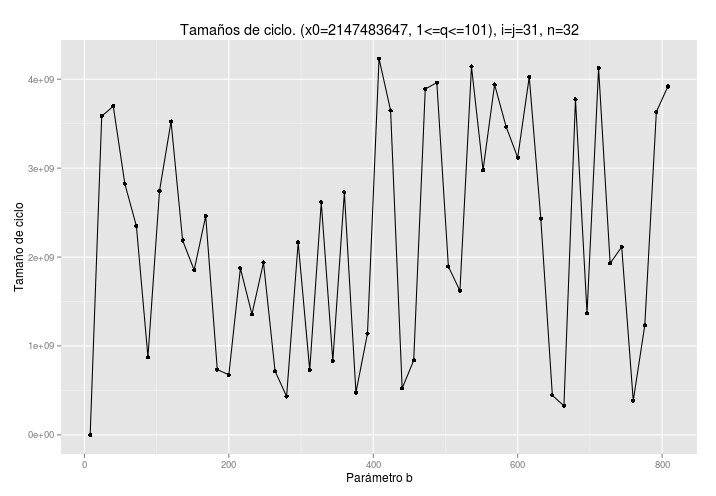
\includegraphics[width=15cm]{ozi.jpeg}}
\caption{Mapa caótico Renyi.} \label{Param}
\end{figure}

De acuerdo a la gráfica anterior, \textbf{un valor de q adecuado para este caso es el siguiente: $400 \leq q \leq 600$}.


\subsection{Ejemplo 1. $i=j=5, n=32$}

Ahora, vamos a  relaizar otra prueba, en este caso $i=j=5$, los resultados obtenidos son los siguientes. 


\begin{figure}[H]
\centering
\subfigure{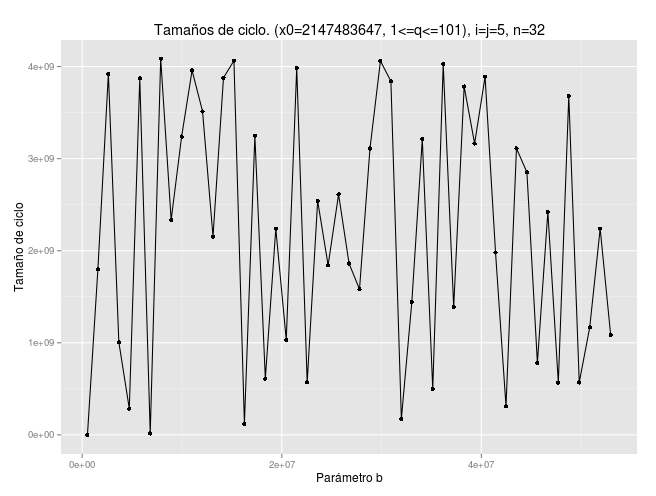
\includegraphics[width=15cm]{ka.jpeg}}
\caption{Mapa caótico Renyi.} \label{Param}
\end{figure}

Hay muchos tamaños de ciclo que son muy grandes, sin embargo, no se puede identificar un patrón específico respecto al valor de q y el cálculo de parámetro.




\section{Referencias.}


\bibliographystyle{plain}
\bibliography{sample.bib}



\end{document}

